\documentclass[11pt]{article}

\usepackage[left=3cm,right=3cm,top=3cm,bottom=3cm]{geometry}
\usepackage{listings}
\usepackage[usenames, dvipsnames]{color}
\usepackage{scrextend}
\usepackage{multicol}
\usepackage{amsthm}
\usepackage{enumitem}
\usepackage{tikz}
\usepackage{bm}
\usetikzlibrary{decorations.pathmorphing}
\usepackage{amsfonts}
\usepackage{amsmath}
\usepackage{ulem}
\usepackage{pdfpages}
\usepackage{graphicx}
\usepackage{subcaption}
%%\usepackage{natbib}

%%\setlength{\bibsep}{1pt}
\setlength{\parindent}{0em}
\setlength{\parskip}{1em}
\lstset{frame=tb,
  language=Haskell,
  aboveskip=3mm,
  belowskip=3mm,
  showstringspaces=false,
  columns=flexible,
  basicstyle={\fontsize{11}{13}\ttfamily},
  numbers=none,
  numberstyle=\tiny\color{Orange},
  keywordstyle=\color{Aquamarine},
  commentstyle=\color{CadetBlue},
  stringstyle=\color{BlueViolet},
  breaklines=true,
  breakatwhitespace=true,
  tabsize=4
}
\newtheorem{lemma}{Lemma}
\newtheorem{example}{Example}
%% (other macros, packages and definitions go here)

\begin{document}
\title{
\vspace{-2em}
  \raggedright
  \textbf{What Happened \\During the Global Financial Crisis?} \\
  \vspace{0.3em}
  \large A brief report on the stock price (financial, tech, energy) in the 2007-09 financial crisis \\
  %\hspace*{\fill}
  \vspace{1em}
  \textit{By} \textbf{Qin Yu}, Jun 2018. 
}
\date{}
\maketitle

%%%%%%%%%%%%%%%%%%%%%%%%%%%%%%%%%
\vspace{-5em}
\hspace{10em}
\parbox[position]{30em}{\textit{The financial crisis of 2007–2008, also known as the global financial crisis and the 2008 financial crisis, is considered by many economists to have been the worst financial crisis since the Great Depression of the 1930s.\cite{Wiki}}}


\section{Introduction: the Data}\vspace{-1em}
To analyse the stock price data, statistically, during the Global Financial Crisis, the auther used R on selected once including 8 stocks for the financial industry (and the average), 4 stocks for the technology industry, and 4 stocks for the energy industry, from $1^{st}$ July 2006 to $30^{th}$ june 2011 (but focus on $1^{st}$ Jan. 2007 to $31^{st}$ Dec 2010). With illustrations, we shall see from a mathematical and statistical point of view, what happend to these industries in the Global financial crisis.
\begin{center}
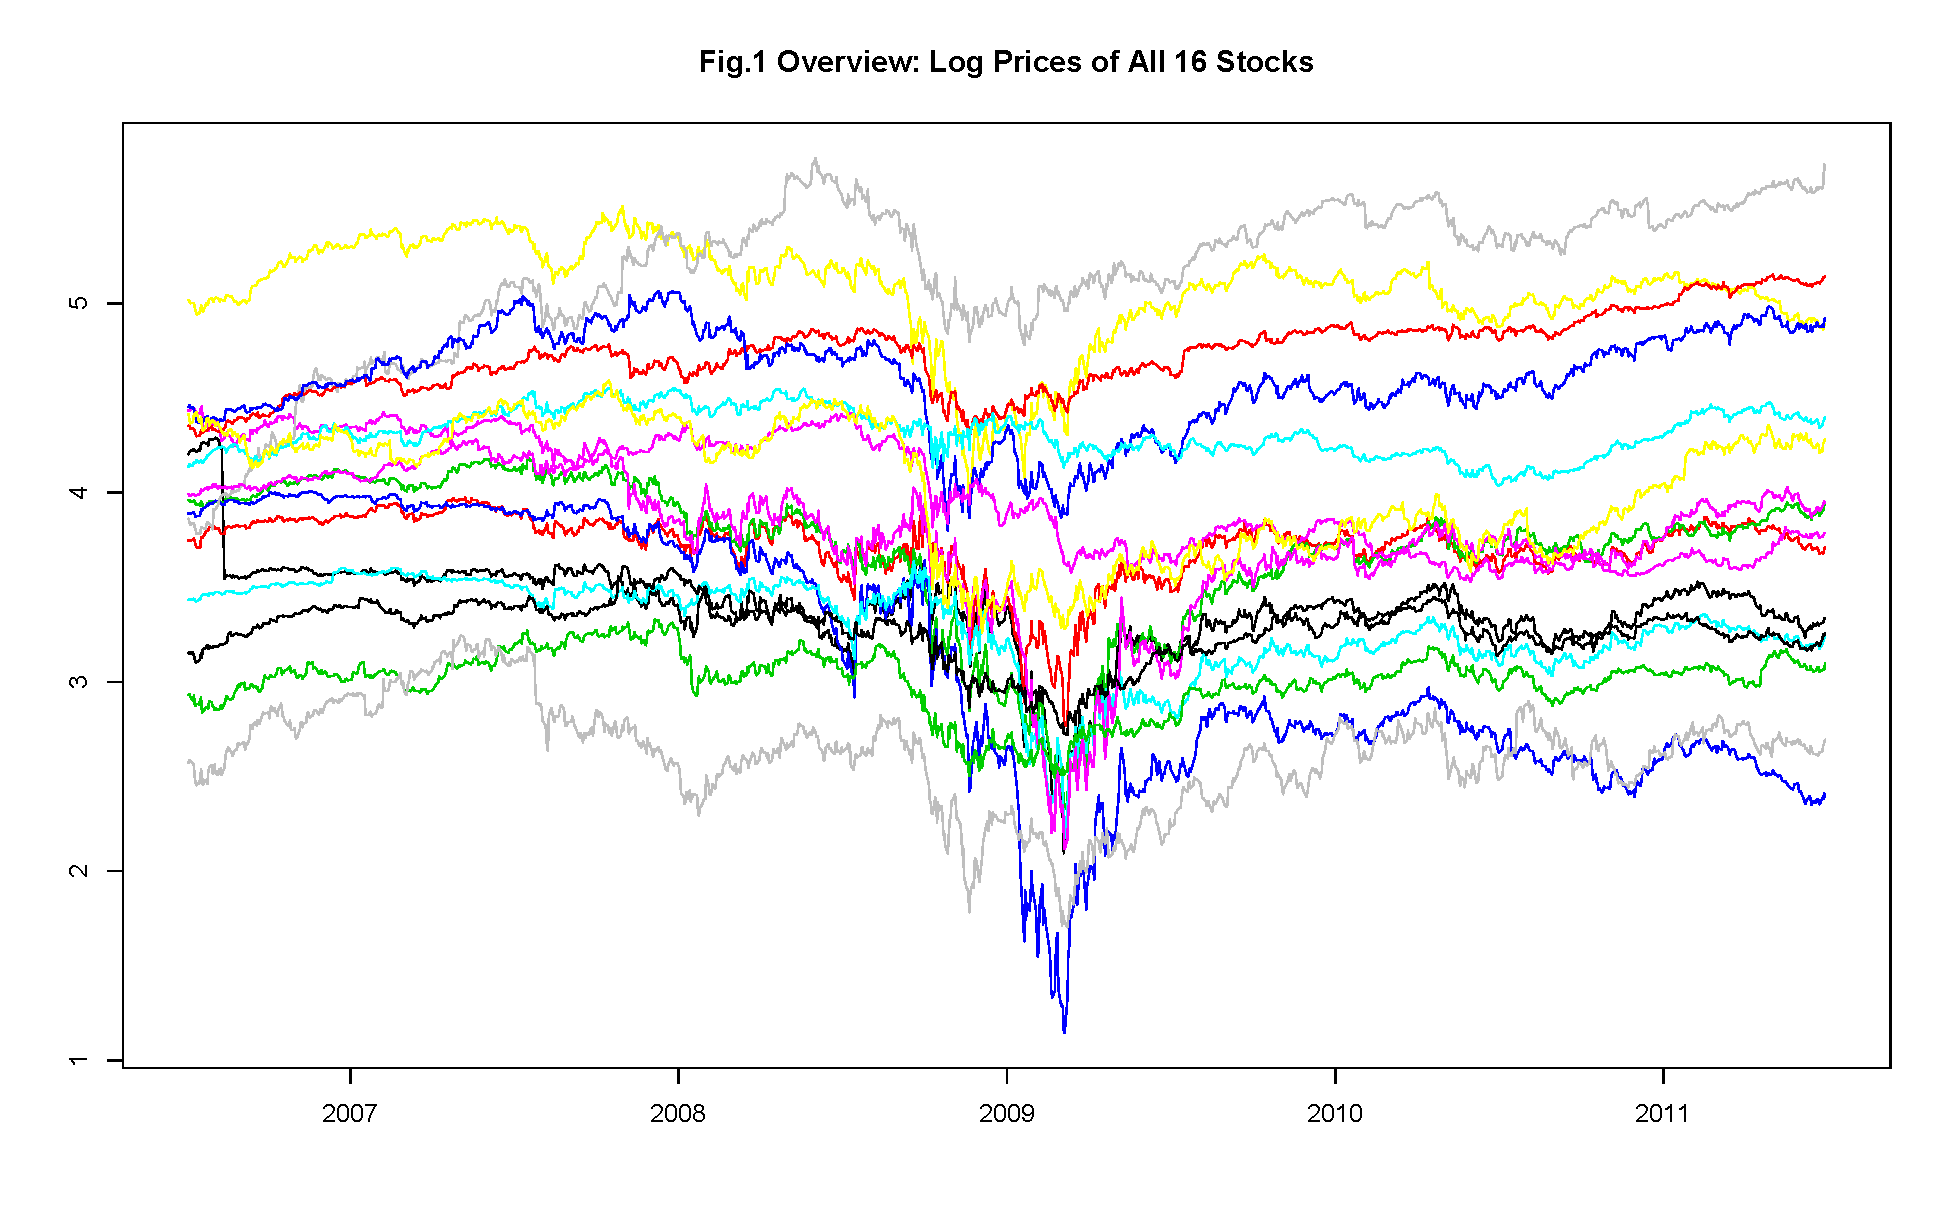
\includegraphics[width=1\linewidth]{graph/Fig1OverviewLogPricesOfAll16Stocks.pdf}
\end{center}


\section{Overview: the Dynamics}\vspace{-1em}
From Figure 1, 2, 3 and 4, one observes the early tremors started around Febrary 2007. and June 2007 is when things really went wrong as we see clearly in both figures. Here is some key dates and eventsrelated to the graph:
\begin{description}\vspace{-1em}
\item[Jun. 2008] There is a sign of an undesirable trend, and this is when the subprime mortgage crisis happened: ``Two Bear Stearns-run hedge funds with large holdings of subprime mortgages run into large losses and are forced to dump assets. The trouble spreads to major Wall Street firms such as Merrill Lynch, JPMorgan Chase(Fig.2.2 JPM), Citigroup and Goldman Sachs(Fig.2.7 GS) which had loaned the firms money''\cite{Guillen}.
\item[22 Jan. 2008] The situation seems to be in control briefly as ``the Federal Reserve System (The Fed) stepped in''\cite{Jolly}.
\item[14 Mar. 2008] ``Global investment bank Bear Stearns becomes a major early casualty and is bought by JP Morgan(Fig.2.2 JPM) for \$240m''\cite{Jolly}. This is ``orchestrated by and backed by the US government, following a sharp decline in shares and a collapse in the confidence in the company''\cite{Guillen}.
\item[15 Sep. 2008] The market fell apart, all stock went down: ``The Dow Jones Industrial average plunges 504 points to close at 10,917.51''\cite{Guillen}. ``Investment bank Lehman Brothers files for the largest bankruptcy in history. Panic breaks out in markets across the world as massive leverage overwhelms a bank with \$639bn in assets. The next day the Fed is forced into an \$85bn bailout of American International Group (AIG)''\cite{Jolly}.
\end{description}
\begin{center}
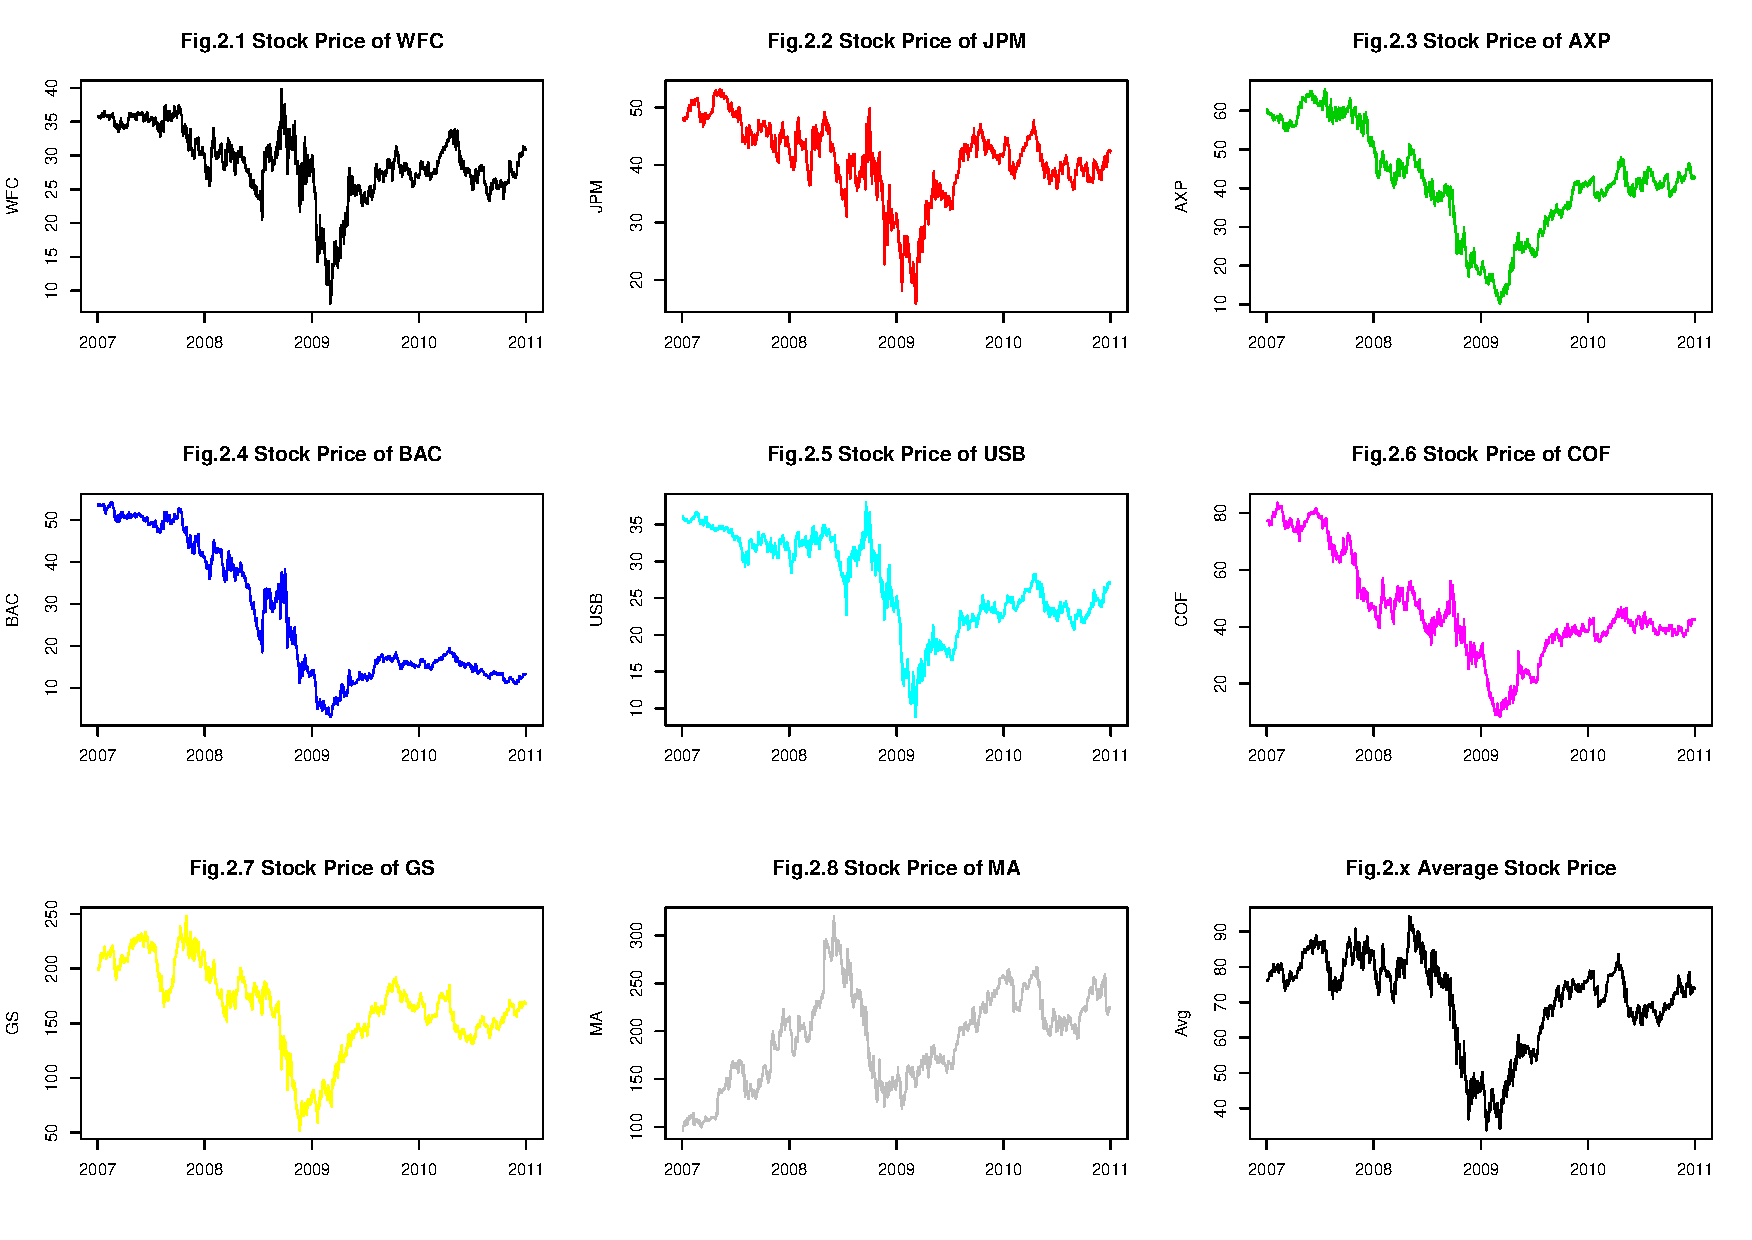
\includegraphics[width=0.95\linewidth]{graph/FinancialStockPrice.pdf}
\end{center}
\begin{center}
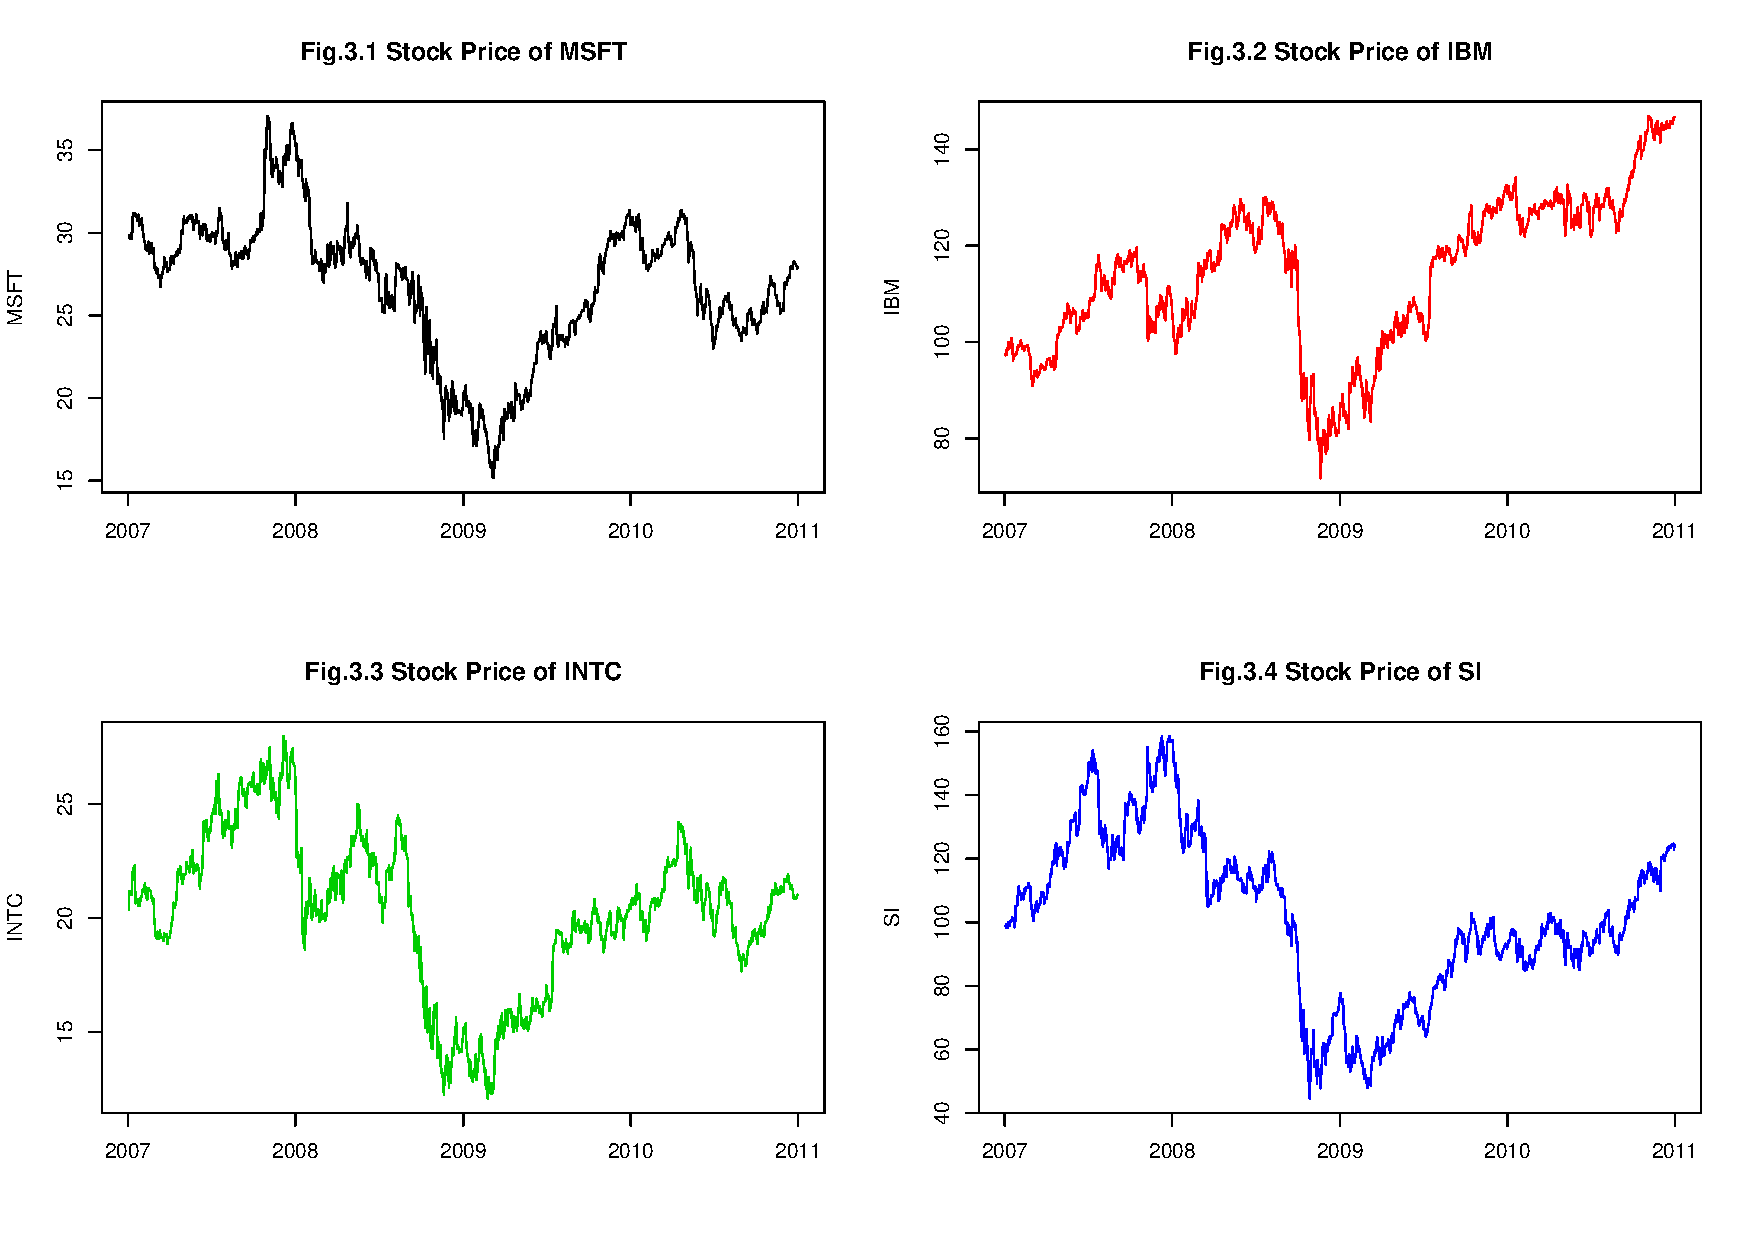
\includegraphics[width=0.85\linewidth]{graph/TechStockPrice.pdf}
\end{center}\vspace{-1em}
\begin{description}\vspace{-1em}
\item[Oct. 2008] Emergency Economic Stabilization Act was signed into law in US, Iceland’s financial sector collapsed, UK government to stepped in to shield British depositors, and so on. Governments around the world made every effort trying to stop the chaos but nothing could bring the broken market back to life. As we see in all figures, all stocks plunged until 2009.
\end{description}\vspace{-1em}
\begin{center}
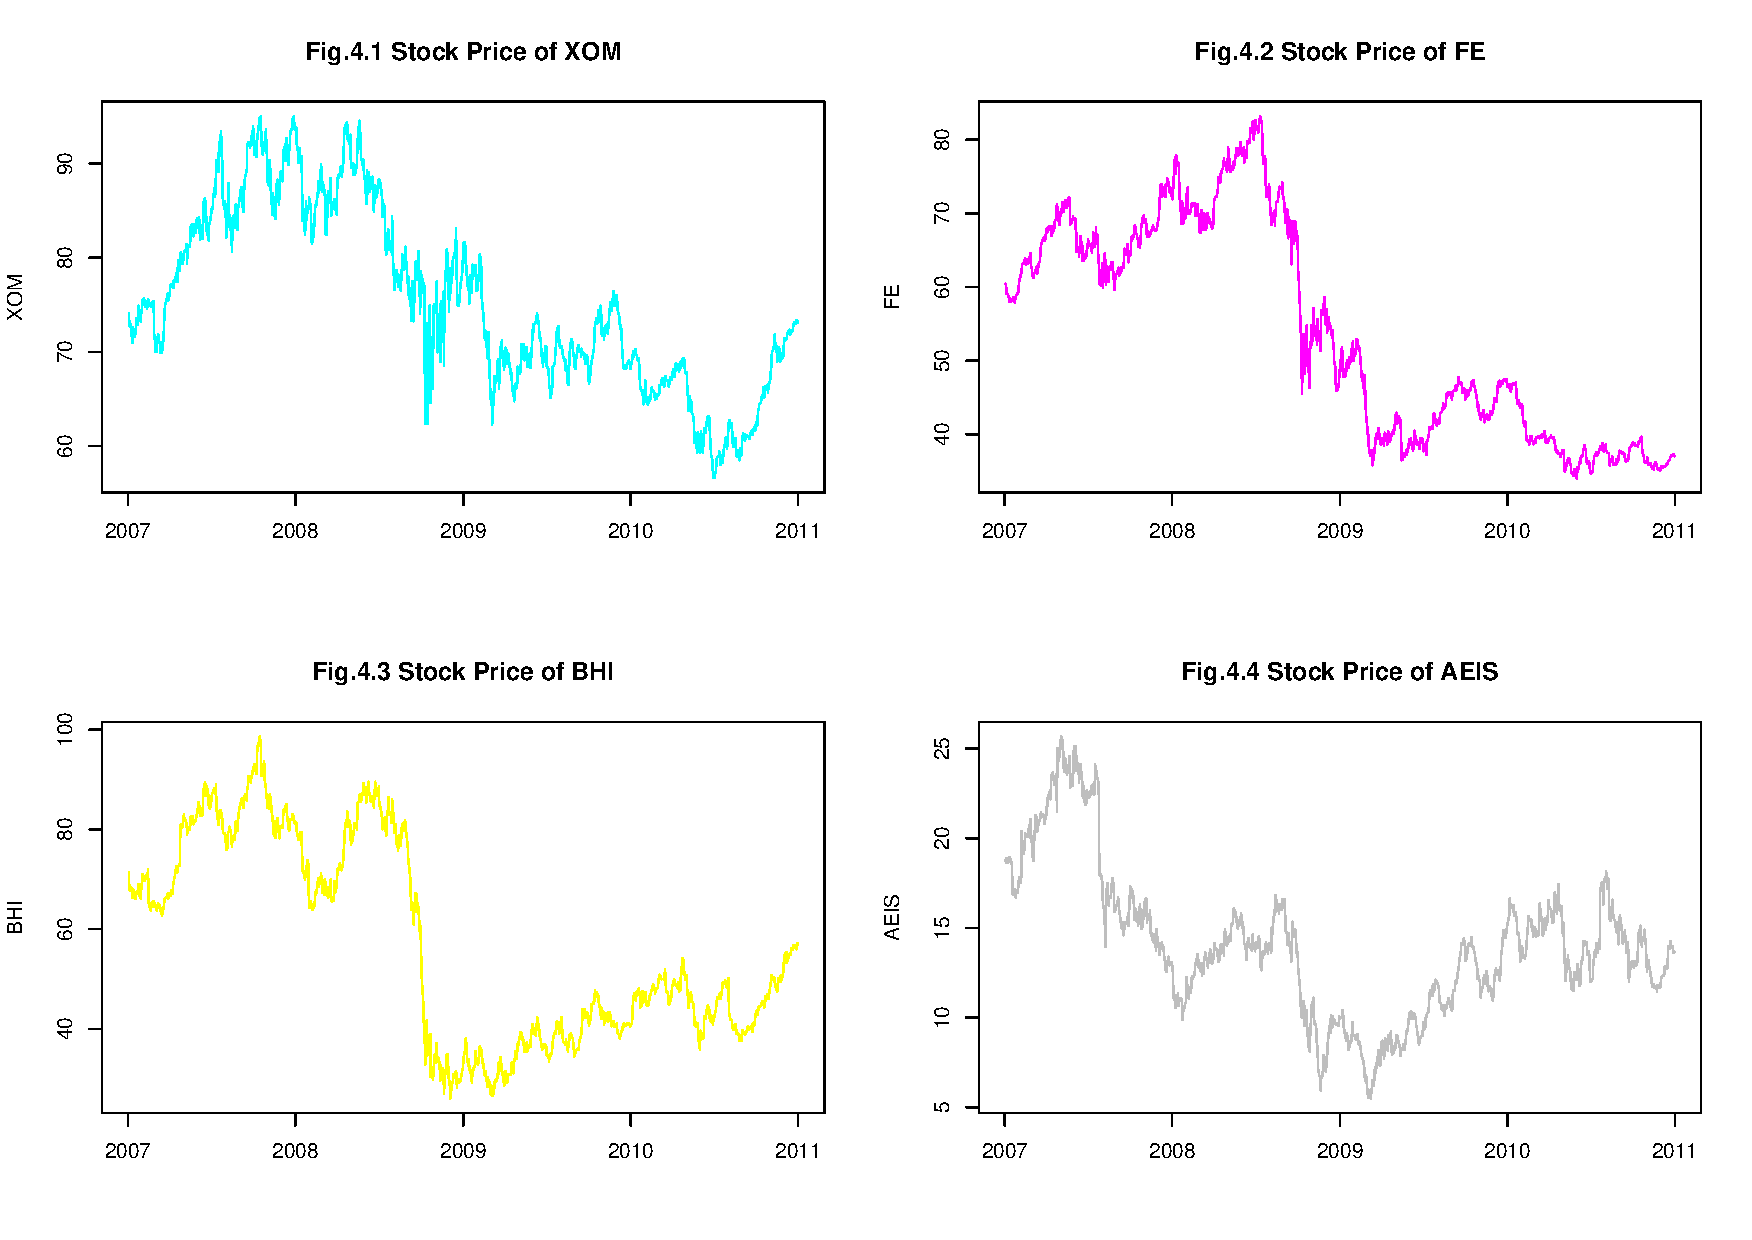
\includegraphics[width=0.85\linewidth]{graph/EnergyStockPrice.pdf}
\end{center}
%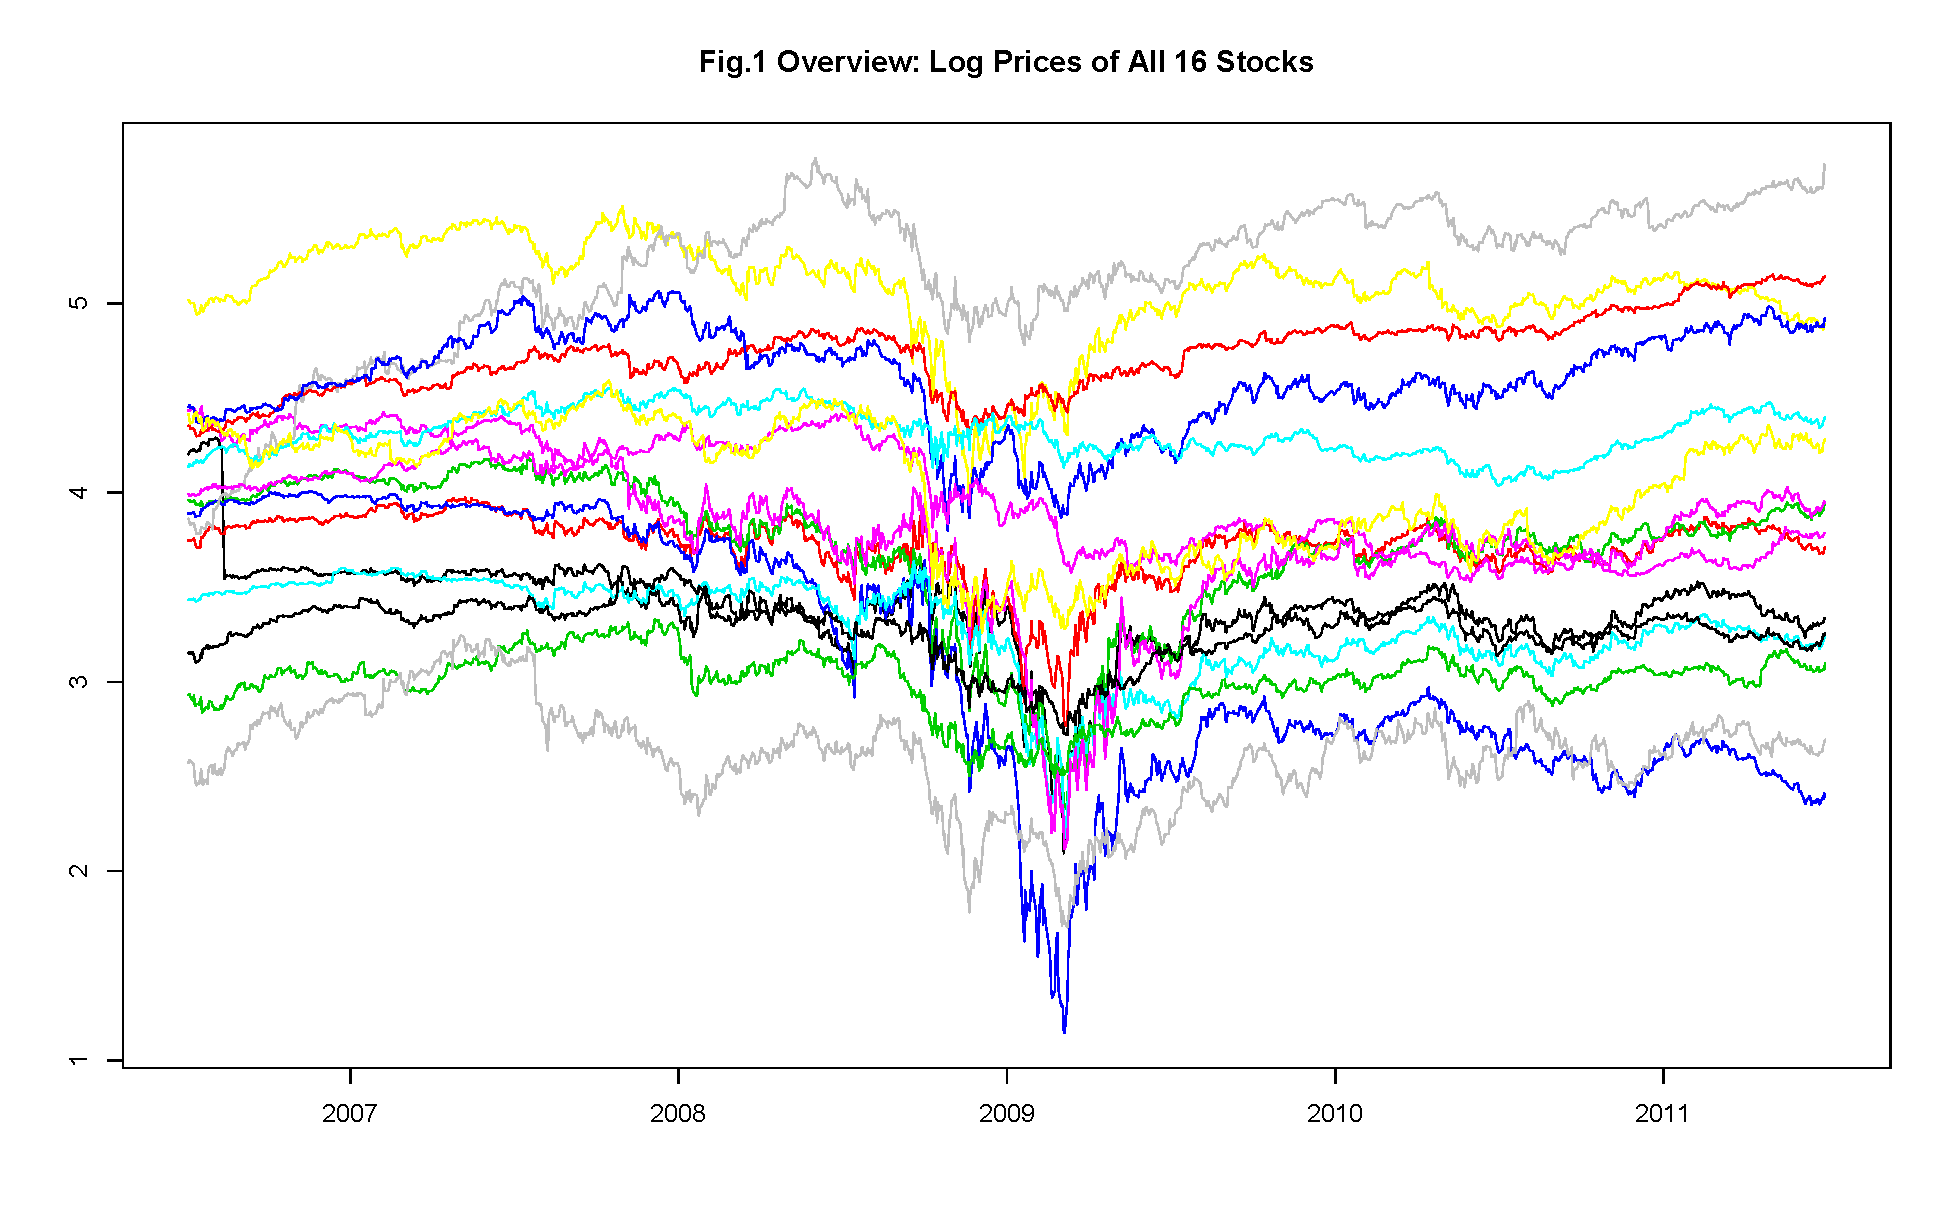
\includepdf[scale=0.9, pages=-, landscape=true]{graph/Fig1OverviewLogPricesOfAll16Stocks.pdf}
%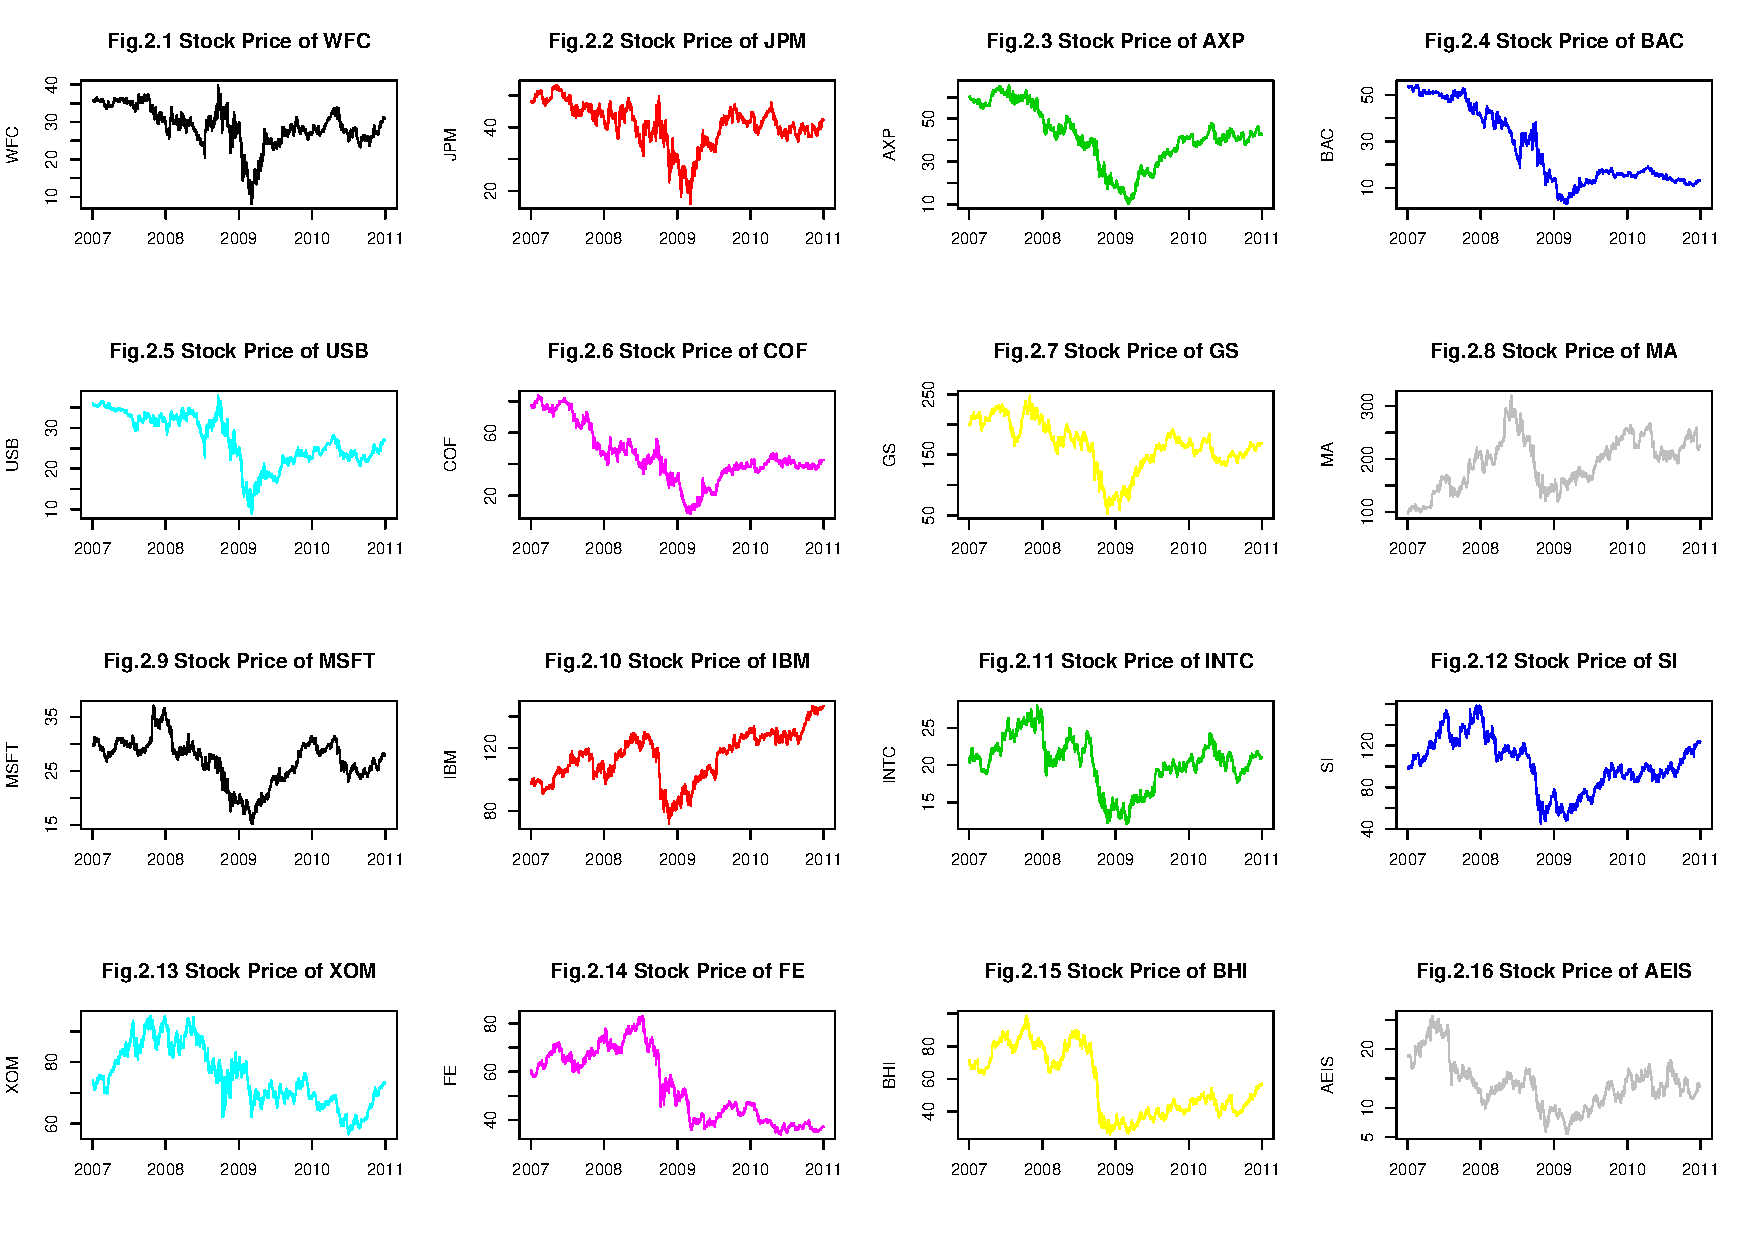
\includepdf[scale=0.9, pages=-, landscape=true]{graph/Fig2StockPriceDynamics.pdf}


\section{Analysis of Dependencies}\vspace{-1em}
How are stocks correlated, from the same sector and different sectors respectively? In the following illustration, pies and shades are symmetric along the labelled diagonal. Percentages and sharpness of blue represent strength in (positive) correlations (since there are no negatively correlated stocks here which should be red if they exist). 
\vspace{-2em}
\begin{center}
  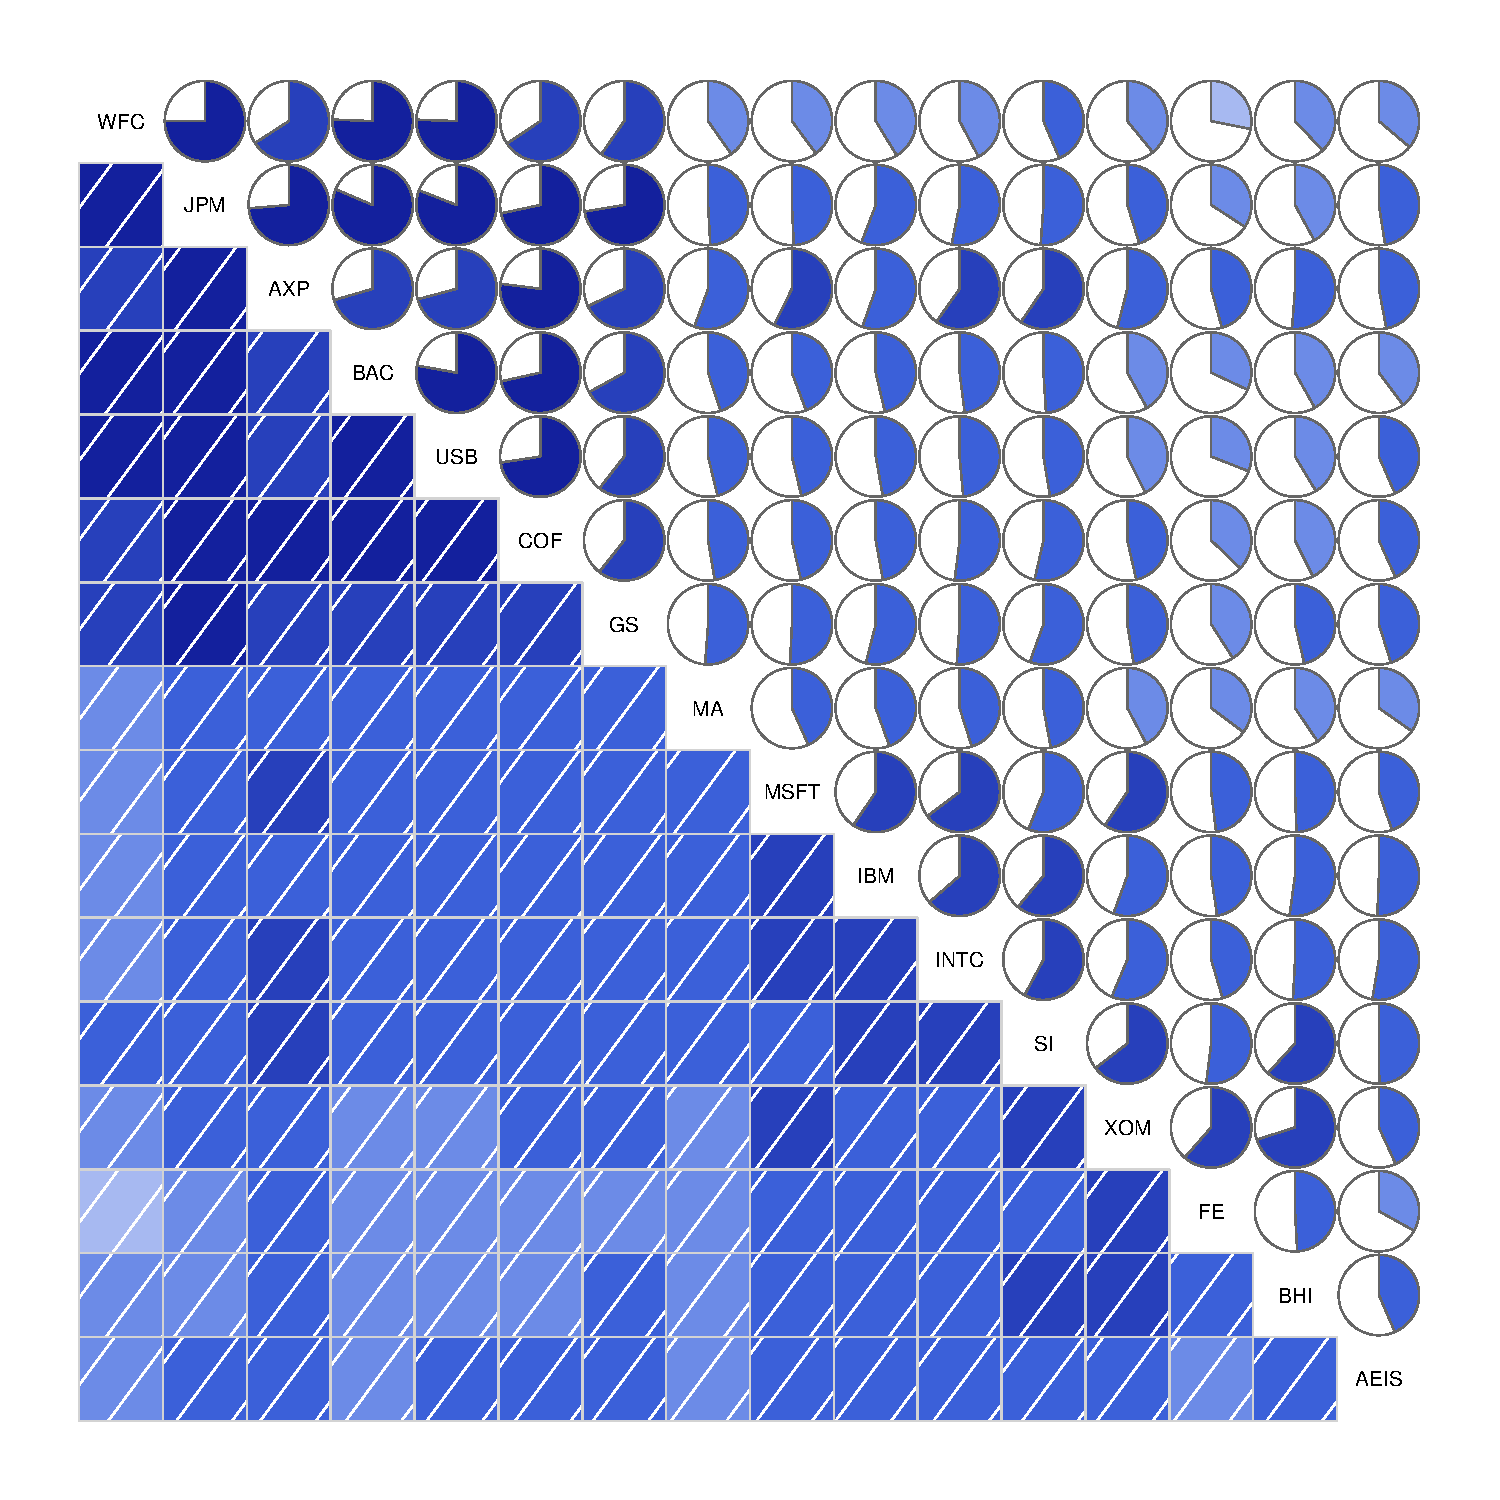
\includegraphics[width=1\linewidth]{graph/PairWiseScatterPlotForAllPie.pdf}\vspace{-1em}\\
  Fig.5 Pairwise Scatter Plot for Log Price of All 16 Stocks\\ 1-8 Financial, 9-12 Tech, 13-16 Energy
\end{center}

\subsection{Correlation Across Sectors}\vspace{-1em}
For correlations across sectors we look at the top-right and bottom-left quarters, as well as that of the bottom-right quarter. Grids representing these correlations are blue but relatively bright and low in percentage, which, statistically, shows all the sectors are weakly correlated but still have positive influence. In English, these three sectors all had a bad time during the global financial crisis but had different levels and periods of losses.
\begin{description}\vspace{-1em}
\item[Financial vs Technology] moderate correlation
\item[Technology vs Energy] moderate correlation
\item[Energy vs Financial] weak correlation
\end{description}

\subsection{Correlation Within Sector}\vspace{-1em}
The correlation between stocks in the same sector is substantial as indicated by the deep blue grids/high percentage pies around each sector. 
\begin{description}\vspace{-1em}
\item[Financial Sector] Inspecting the top-left quarter of Fig.5, i.e. the Financial sector, one can easily tell the \textbf{strong} link between financial stocks.
\item[Technology Sector] The 10 grids for Technology sector are blue with \textbf{relatively strong} hue, suggesting good dependencies between companies in this industry.
\item[Energy Sector] \textbf{Weak-to-modest} correlation is shown within Energy sector.
\end{description}
  

\section{Testing Portfolio and Loss Distribution}\vspace{-1em}
Suppose there is a portfolio which invests \$1000 in each of the stocks at $1^{st}$ Jan. 2007 with fixed composition, the empirical data results in Value-at-Risk (VaR) being 637.9547 and Expected Shortfall (ES) being 1037.473. Comparing it to a normal distribution (with VaR being 726.7265 and ES being 910.1906) and the empirical distribution of 2010, we have Fig.6 and 7.
\begin{figure}[h]
\begin{subfigure}{0.33\textwidth}
  \centering
  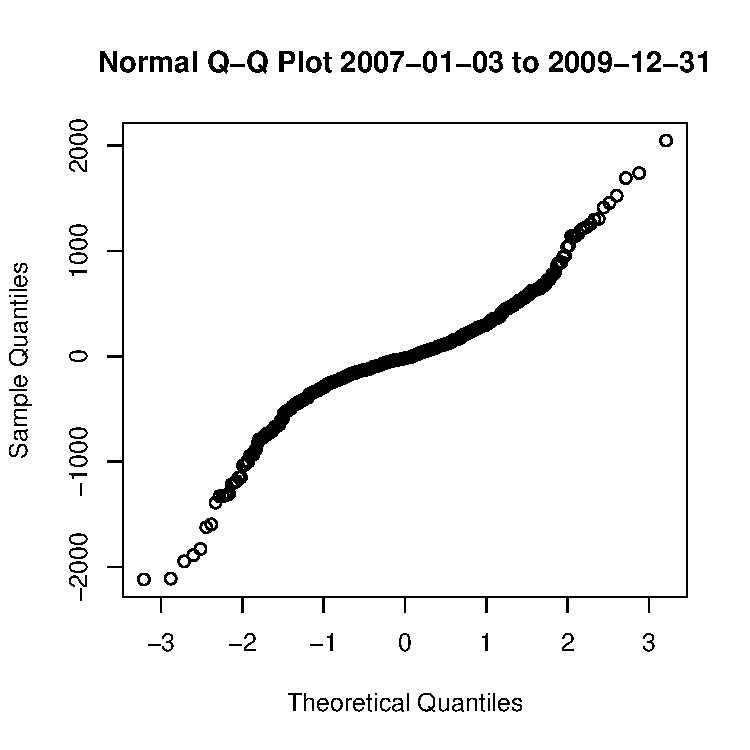
\includegraphics[width=1\linewidth]{graph/NormalQQPlot200709sq.pdf}
\end{subfigure}%
\begin{subfigure}{0.33\textwidth}
  \centering
  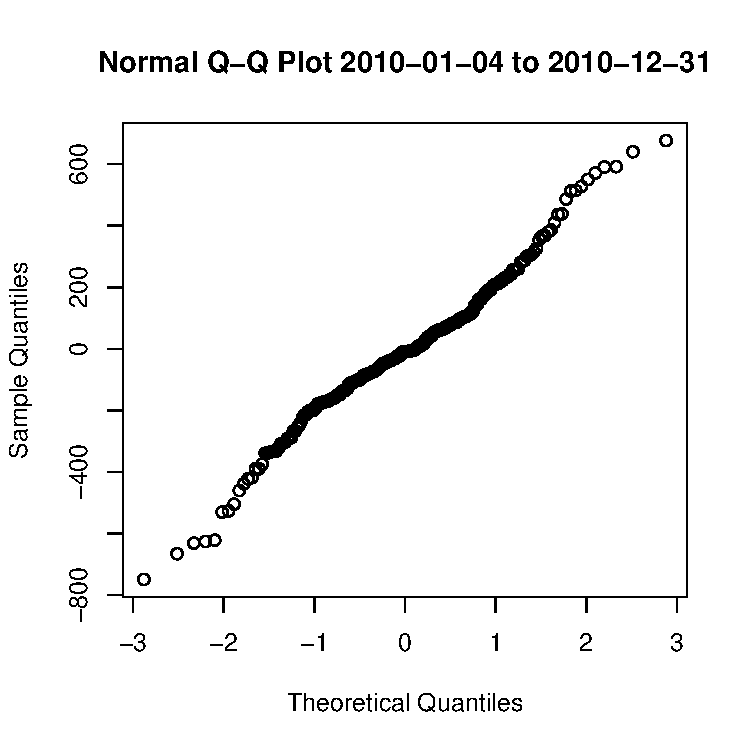
\includegraphics[width=1\linewidth]{graph/NormalQQPlot2010sq.pdf}
\end{subfigure}
\begin{subfigure}{0.33\textwidth}
  \centering
  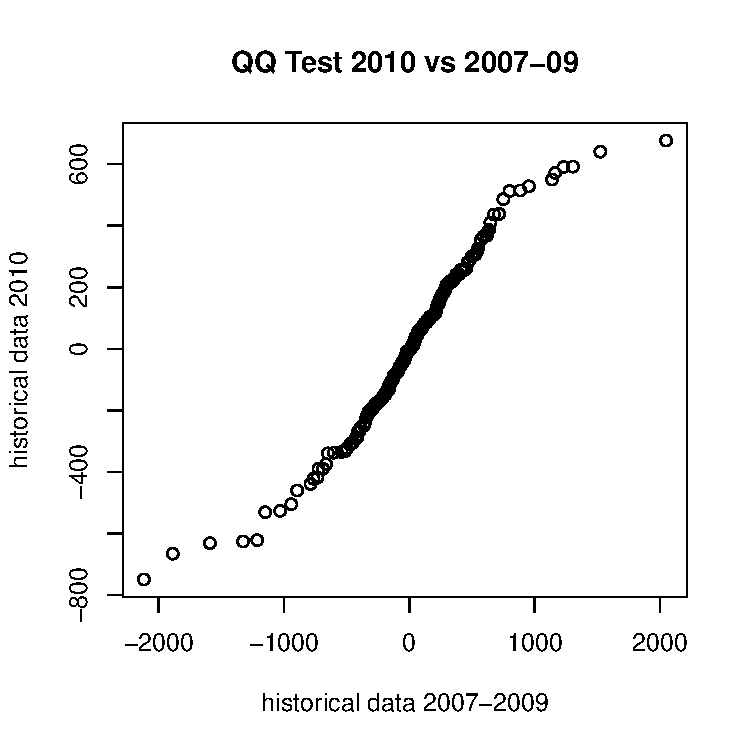
\includegraphics[width=1\linewidth]{graph/QQ200709against2010sq.pdf}
\end{subfigure}
\centering Fig.6 Normality Test and Q-Q Plot
\end{figure}

\vspace{-1em}\subsection{Quantile-quantile Plot}\vspace{-1em} 
In this quantile-quantile plot (Fig.6.1) of daily returns of the portfolio, the inverted-S shape means that the empirical distribution has a heavier tail than the normal distribution, i.e. the data have more extreme values than what would be expected if they truly came from a Normal distribution. However, the subsequent data for 2010 is closer to normal as we see in Fig.6.2. Also, the Q-Q plot of 2010 against 2007-09 shows that data in 2010 has less extreme values. As a result, the model obtained from 2007-09 is not suitable for 2010 data.

\vspace{-1em}\subsection{VaR and ES}\vspace{-1em}
Comparing two distributions in Fig.7, it is clear that 2010 data is more stable and has smaller VaR and ES. To examine this more closely:
\begin{align*} 
  &\text{VaR}_{0.95}(L_{2007/09})& &=& &637.9547& \\
  &\text{VaR}_{0.95}(L_{2010})& &=& &396.7451& \\
  &\text{ES}_{0.95}(L_{2007/09})& &=& &1037.473& \\
  &\text{ES}_{0.95}(L_{2010})& &=& &534.4695& \\
\end{align*}
\vspace{-2.5em}
\begin{figure}[h]
\begin{subfigure}{0.5\textwidth}
  \centering
  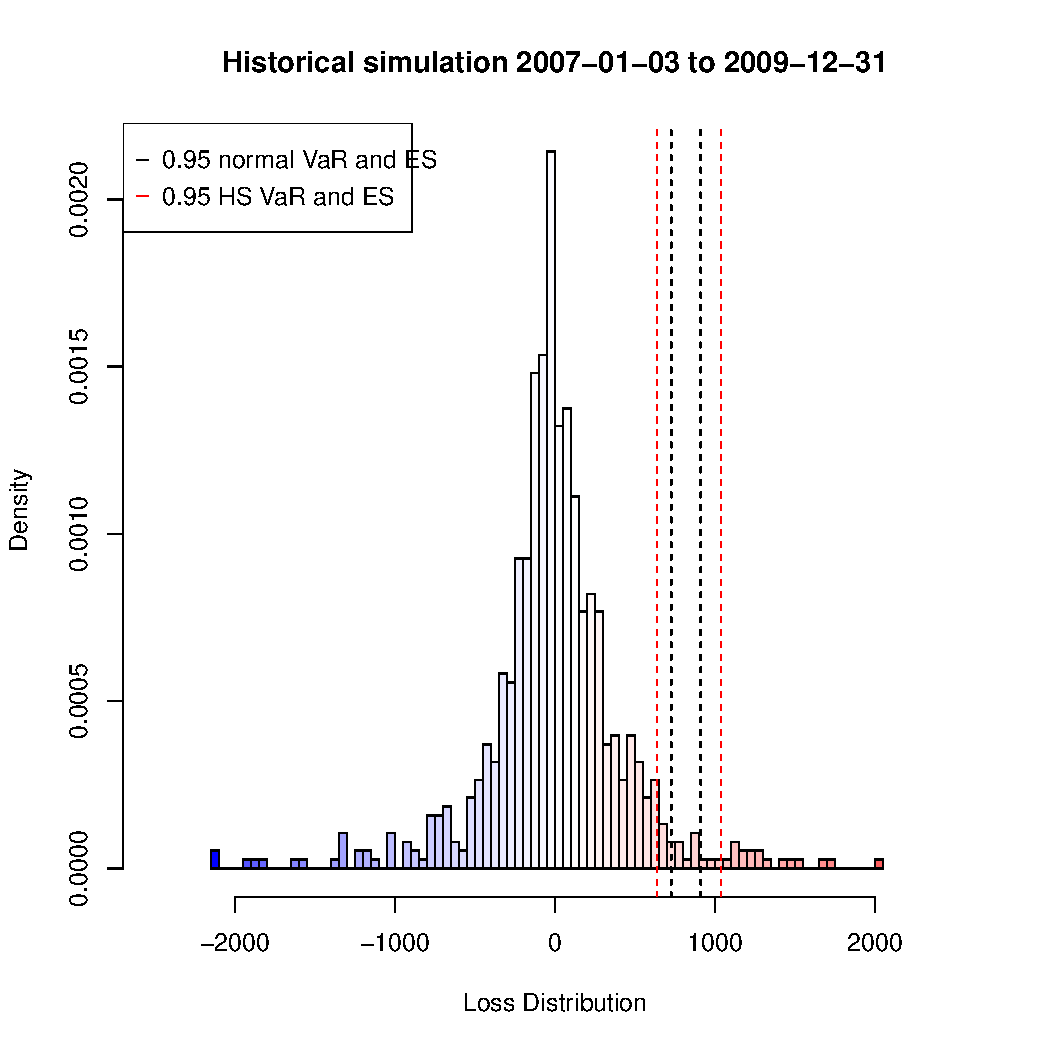
\includegraphics[width=1\linewidth]{graph/HistoricalSimulation200709sq.pdf}
\end{subfigure}%
\begin{subfigure}{0.5\textwidth}
  \centering
  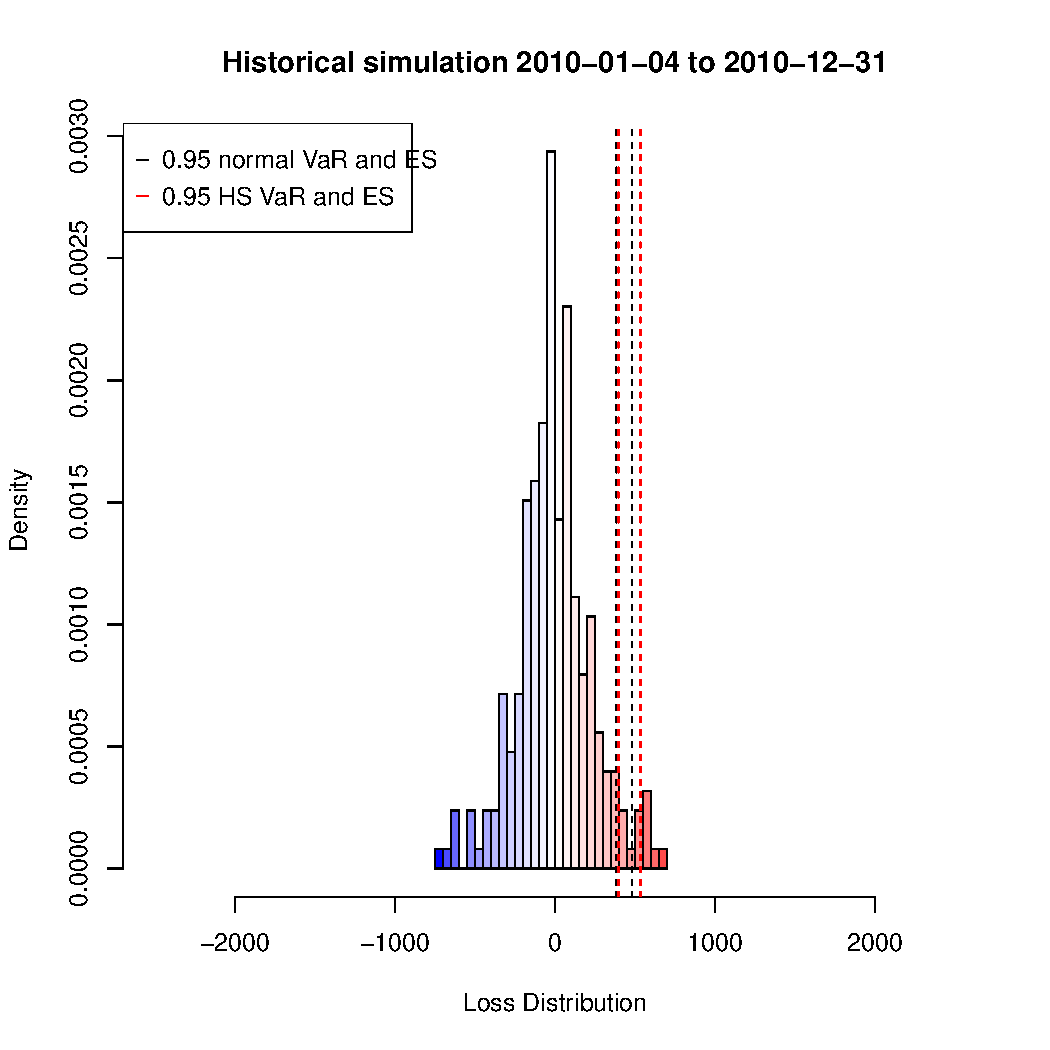
\includegraphics[width=1\linewidth]{graph/HistoricalSimulation2010sq.pdf}
\end{subfigure}
\centering Fig.7 VaR and ES
\end{figure}


\section{Dependencies and Copulae}\vspace{-1em}
\begin{center}
  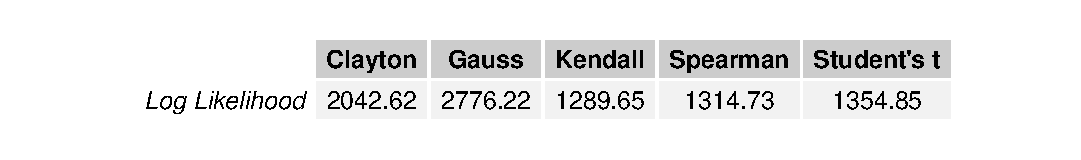
\includegraphics[width=1\linewidth]{graph/LogLikelihood.pdf}
  Table.8 Log Likehoods for 5 copulae (Gumbel is only implemented for d = 2)
\end{center}
By computing the log likelihood for 5 copulae: Clayton, Gauss, Kendall, Spearman, and Student's t, we can see that the best fit copula is the Gauss Copula. Also, Fig.9 illustrates the relatively thin bands in the correlations plotted.
\begin{center}\vspace{-1em}
  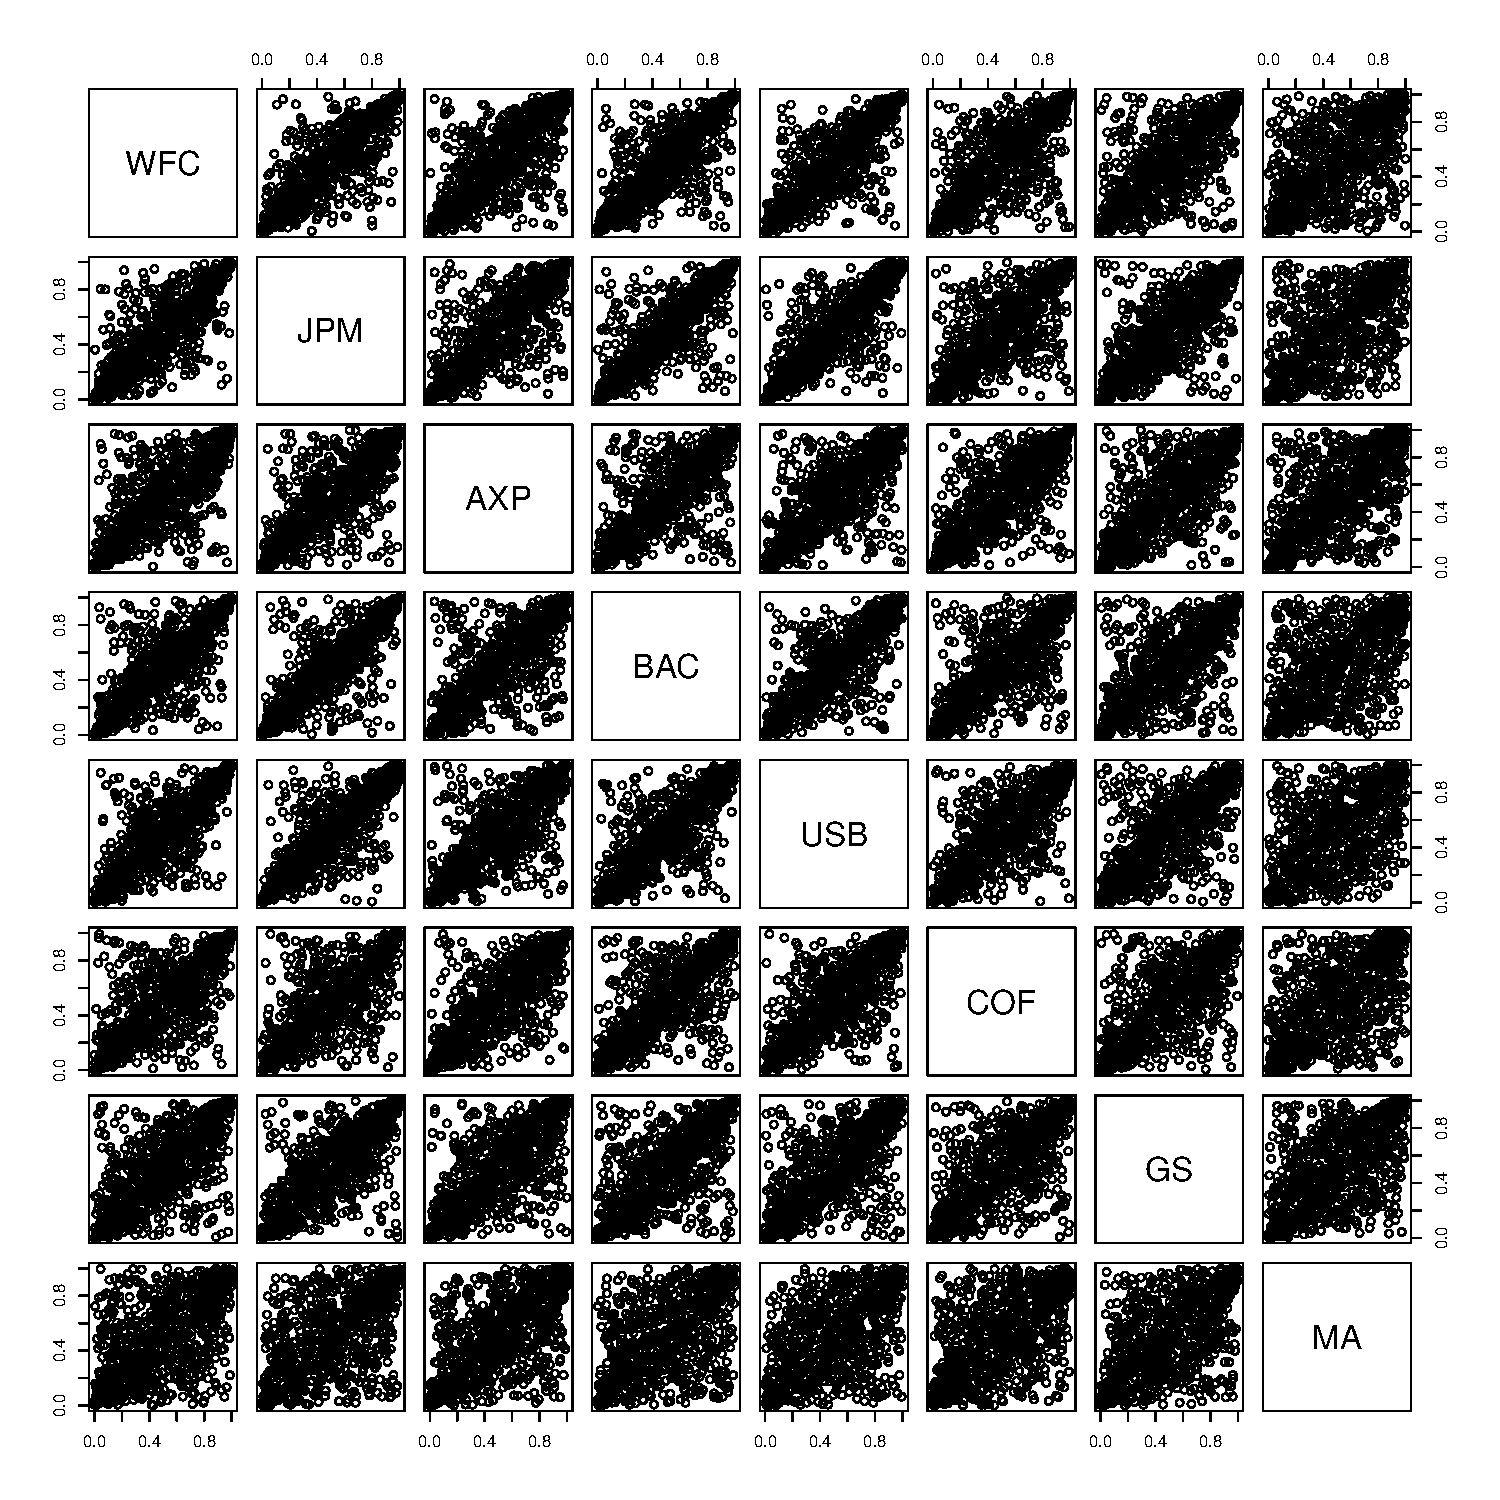
\includegraphics[width=1\linewidth]{graph/CopulaY.pdf}
  Fig.9 Scatter Plot of Copulae
\end{center}


\section{Conclusion}\vspace{-1em}
During the Global Financial Crisis, the financial, technology and energy sectors all experienced destructive depression. They are all positively related to a high level, especially within the same industry. Diversification is still helpful in this situation but as the whole market fell apart there is no escape. Finally, the data obtained from previous periods is not helpful for determining possible trends.


%%%%%%%%%%%%%%%%%%%%%%%%%%%%%%%%%
\vspace{-0.8em}
\begin{thebibliography}{9}
\bibitem{Wiki} Wikipedia contributors. ``Financial crisis of 2007–2008.'' Wikipedia, The Free Encyclopedia. Wikipedia, The Free Encyclopedia, 29 Jun. 2018. Web. 30 Jun. 2018.
\bibitem{Guillen} Guillén, Mauro F. ``The global economic \& financial crisis: A timeline.'' The Lauder Institute, University of Pennsylvania (2009): 1-91.
\bibitem{Jolly} Jolly, J. (2017). ``The financial crisis 10 years on: A timeline of the crash.'' [online] Cityam.com. Available at: http://www.cityam.com/269810/global-financial-crisis-10-years-timeline-global-events [Accessed 30 Jun. 2018].
\end{thebibliography}
%%%%%%%%%%%%%%%%%%%%%%%%%%%%%%%%%
\end{document}
